\documentclass[aspectratio=169,
hyperref={colorlinks,urlcolor=blue}
]{beamer}


%\usetheme{Pittsburgh}
\usetheme{default}
\usepackage{colortbl}%colored tables
%For using helvetica font:
\usepackage[scaled]{helvet}
\usepackage[T1]{fontenc}
\renewcommand\familydefault{\sfdefault}
\urlstyle{same} %sets the fonts for urls
\usepackage{pdfpages}
\usepackage{siunitx}
\usepackage{caption}
\usepackage{pifont}%for dings
\usepackage{pgfplots}%for 3d plotting
\pgfplotsset{compat = newest}
\usepackage{mathtools}%box in align env \Aboxed
\usepackage[american,smartlabels]{circuitikz}%for drawing circuits
\usepackage{multimedia}
\usepackage{animate}
\usepackage{xcolor}


\usetikzlibrary{arrows}
\usetikzlibrary {3d} 
\usetikzlibrary{decorations.markings, math}
\usetikzlibrary{intersections, pgfplots.fillbetween}
\usetikzlibrary {shapes.geometric} 


%\definecolor{myblue}{RGB}{5, 34, 150}
\definecolor{myblue2}{RGB}{5, 34, 150}
\definecolor{myblue}{RGB}{0,36,82}
\definecolor{myred}{RGB}{207, 2, 13}
\definecolor{mygreen}{RGB}{0, 158, 11}
\definecolor{myyellow}{RGB}{220,220,0}
\definecolor{qblue}{RGB}{0,36,82}
\definecolor{qgold}{RGB}{250,189,15}
\definecolor{qred}{RGB}{185,14,49}
\definecolor{cblue}{rgb}{0.13, 0.67, 0.8}
\definecolor{corange}{rgb}{0.8, 0.34, 0.0}
\definecolor{cpurple}{rgb}{0.54, 0.29, 0.42}

%%%%%%%%%%%% General settings
\setbeamercolor{frametitle}{fg=black}
\setbeamercolor{title}{fg=black}
\setbeamercolor{author}{fg=myblue2}

\beamertemplatenavigationsymbolsempty %no navigation controls at bottom of slides
%\setbeamertemplate{footline}[frame number]
\usefonttheme{professionalfonts} 
\setbeamerfont{title}{series=\bfseries,parent=structure}
\setbeamerfont{frametitle}{series=\bfseries,parent=structure}

%%%%%%%%%%%%Lists
\setbeamertemplate{itemize item}[circle] %{\color{myblue}$\circ$}
\setbeamertemplate{itemize subitem}{\color{myblue2}$\circ$}
\setbeamertemplate{itemize subsubitem}{\color{myblue2}$\cdot$}
\setbeamercolor{itemize item}{bg=myblue2,fg=myblue2}
\setbeamercolor{enumerate item}{bg=myblue2,fg=myblue2}
%%%%%%%%%%%%%%%%%%%%%%%%%%%%

%%%%%%%%%%%%Blocks
\setbeamertemplate{blocks}[rounded]
%Default block
\setbeamercolor{block title}{bg=myblue2, fg=white}
\setbeamercolor{block body}{bg=myblue2!10}
\setbeamerfont{block body}{size=\scriptsize}
\setbeamerfont{block title}{size=\scriptsize}
%Alert block
\setbeamercolor{block title alerted}{bg= myblue2, fg=white}
\setbeamercolor{block body alerted}{bg=myblue2!10}
\setbeamerfont{block body alerted}{size=\scriptsize}
\setbeamerfont{block title alerted}{size=\scriptsize}
%example block
\setbeamercolor{block title example}{bg=mygreen, fg=white}
\setbeamercolor{block body example}{bg=mygreen!10}
\setbeamerfont{block body example}{size=\scriptsize}
\setbeamerfont{block title example}{size=\scriptsize}
%%%%%%%%%%%%%%%%55


%%%%%%%%%%%%Figures and captions
\captionsetup{font=scriptsize,labelfont=scriptsize}
%\setbeamertemplate{caption}{\raggedright\insertcaption\par}
\newenvironment{capfig}[3]{\begin{figure}\includegraphics[width=#1\textwidth]{#2}\caption*{\textit{#3}}\end{figure}}{}

%\makeatother
%\setbeamertemplate{footline}
%{
%  \leavevmode%
%  \hbox{%
%  \begin{beamercolorbox}[wd=.4\paperwidth,ht=2.25ex,dp=1ex,center]{author in head/foot}%
%    \usebeamerfont{author in head/foot}\insertshortauthor
%  \end{beamercolorbox}%
%  \begin{beamercolorbox}[wd=.6\paperwidth,ht=2.25ex,dp=1ex,center]{title in head/foot}%
%    \usebeamerfont{title in head/foot}\insertshorttitle\hspace*{3em}
%    \insertframenumber{} / \inserttotalframenumber\hspace*{1ex}
%  \end{beamercolorbox}
%  }%
%  \vskip0pt%
%}
%\makeatletter

\makeatother
\setbeamertemplate{footline}
{
  \leavevmode%
  \hbox{%
\begin{beamercolorbox}[wd=.27\paperwidth,ht=2.25ex,dp=1ex,center]{author in head/foot}%
    \color{black}{\insertinstitute}
\end{beamercolorbox}
  \begin{beamercolorbox}[wd=.27\paperwidth,ht=2.25ex,dp=1ex,center]{author in head/foot}%
    \color{black}{\inserttitle}
  \end{beamercolorbox}%
  \begin{beamercolorbox}[wd=.27\paperwidth,ht=2.25ex,dp=1ex,center]{title in head/foot}%
    \color{black}{\insertshortauthor}
  \end{beamercolorbox}
  \begin{beamercolorbox}[wd=.27\paperwidth,ht=2.25ex,dp=1ex,center]{title in head/foot}%
    \hspace{.28\paperwidth}\color{black} \insertframenumber{} / \inserttotalframenumber\hspace*{1ex}
  \end{beamercolorbox}
  }%
  \vskip0pt%
}
\makeatletter

\setbeamertemplate{title page}
{
  \begin{tikzpicture}[remember picture,overlay]
    \def\barh{4}%15
  
    \draw[color=myblue2,line width=\barh] ([yshift=-0.5*\barh]current page.north west) -- ([yshift=-0.5*\barh,xshift=-0.67\paperwidth]current page.north east);
    \draw[color=myblue2,line width=\barh] ([yshift=-0.5*\barh,xshift=-0.67\paperwidth]current page.north east) -- ([yshift=-0.5*\barh,xshift=-0.34\paperwidth]current page.north east);
    \draw[color=myblue2,line width=\barh] ([yshift=-0.5*\barh,xshift=-0.34\paperwidth]current page.north east) -- ([yshift=-0.5*\barh]current page.north east); 
  
    \draw[color=myblue2,line width=\barh] ([yshift=0.5*\barh]current page.south west) -- ([yshift=0.5*\barh,xshift=-0.67\paperwidth]current page.south east);
    \draw[color=myblue2,line width=\barh] ([yshift=0.5*\barh,xshift=-0.67\paperwidth]current page.south east) -- ([yshift=0.5*\barh,xshift=-0.34\paperwidth]current page.south east);
    \draw[color=myblue2,line width=\barh] ([yshift=0.5*\barh,xshift=-0.34\paperwidth]current page.south east) -- ([yshift=0.5*\barh]current page.south east);
    %\node[left] at (current page.east) {
    %
\includegraphics[scale=0.1]{figures/coverpage}
    %};
  \end{tikzpicture}
  
  \usebeamerfont{title}\usebeamercolor[fg]{title}\inserttitle\par
  \usebeamerfont{subtitle}\usebeamercolor[fg]{subtitle}\insertsubtitle\par
  \vspace{2cm}
  \usebeamerfont{author}\usebeamercolor[fg]{author}\insertauthor\par
  \usebeamerfont{institute}\usebeamercolor[fg]{author}\insertinstitute\par
  \usebeamercolor[fg]{author}\par
  \usebeamercolor[fg]{titlegraphic}\inserttitlegraphic

} 

\setbeamertemplate{frametitle}{%
    \nointerlineskip%
        \par\hspace*{-\dimexpr0.5\paperwidth-0.5\textwidth}\textcolor{myblue2}{\rule{0.33\paperwidth}{6pt}}\textcolor{myblue2}{\rule{0.33\paperwidth}{6pt}}\textcolor{myblue2}{\rule{0.34\paperwidth}{6pt}} 
    \begin{beamercolorbox}[wd=\paperwidth,ht=0.75cm,dp=0.6ex]{frametitle}
        \hspace*{0.5cm}\strut\usebeamerfont{frametitle}\insertframetitle\strut
        %\hrule
    \end{beamercolorbox}%
    %%Line below:
%\par\hspace*{-\dimexpr0.5\paperwidth-0.5\textwidth}\textcolor{myblue}{\rule{\paperwidth}{0.4pt}}
     % <-- calculation of left margin width + rule
     %\textcolor{red}{\noindent\rule{\paperwidth}{2pt}}
}


%%%%%%%%%%%%Frame templates

%Slide with title
\newenvironment{titleframe}[1]
{\begin{frame}\frametitle{#1}\end{frame}}
{}

%Slide with title and itemize list:
\newenvironment{bulletframe}[1]
{\begin{frame}{#1} \itemize}
{\enditemize \end{frame}}

%Slide with two columns 50/50
\newenvironment{twocolframe}[3]
{\begin{frame}{#1}
 \begin{columns}[T]
 \column{0.5\textwidth}#2
 \column{0.5\textwidth}#3
 \end{columns}\end{frame}}{}

%Slide with two columns 60/40 <<<<<<<<<<<<<<<<<<<<<<  This one!
\newenvironment{twocolframesf}[3]
{\begin{frame}{#1}
 \begin{columns}[T]
 \column{0.6\textwidth}#2
 \column{0.4\textwidth}#3
 \end{columns}\end{frame}}{}
 
%Slide with two columns 70/30
\newenvironment{twocolframest}[3]
{\begin{frame}{#1}
 \begin{columns}[T] 
 \column{0.7\textwidth}#2
 \column{0.3\textwidth}#3
 \end{columns}\end{frame}}{} 
 
%Slide with two columns 40/60
\newenvironment{twocolframefs}[3]
{\begin{frame}{#1}
 \begin{columns}[T] 
 \column{0.4\textwidth}#2
 \column{0.6\textwidth}#3
 \end{columns}\end{frame}}{}
 
%Slide with two columns 70/30
\newenvironment{twocolframets}[3]
{\begin{frame}{#1}
 \begin{columns}[T] 
 \column{0.3\textwidth}#2
 \column{0.7\textwidth}#3
 \end{columns}\end{frame}}{} 

 
%Colloquium speaker (title, abstract, picture file, speaker name)
\newenvironment{colloquium}[5]
{
\begin{frame}{Colloquium: Friday 1:30pm in Stirling A}
\begin{columns}[T] 
 \column{0.8\textwidth}
 \textbf{#1}\\
 #2
 \column{0.2\textwidth}
 \capfig{#3}{#4}{#5}
 \end{columns}
\end{frame}
}
{} 

%%%%%%%%%%%%%Set Hyperref colors


\hypersetup{
  colorlinks=true,
  linkcolor=blue,    
  urlcolor=blue,     
  citecolor=blue      
}
%%%%%%%%%%%%%TOC bolding
\setbeamerfont{section in toc}{series=\bfseries}



%Frames:
% \twocolframesf 60/40 (fs, st, ts) 
% \titleframe
% bulletframe


%%%%%%%%%%%%%%%%%%%%%%%%%
%%%%%% START OF PRESENTATION %%%%%%
%%%%%%%%%%%%%%%%%%%%%%%%%

\title{Angular Momentum and Rolling}
\subject{Rotational Energy, Momentum and RWS}
\subtitle{Building Models to Describe our World}


\begin{document}

%%%%%%%%%%%%%%%%%%%%%%%%%
%%%%%% Title slide %%%%%%
%%%%%%%%%%%%%%%%%%%%%%%%%
\chaptertitle{Angular Momentum and Rolling}
\begin{frame}
\titlepage
\thispagestyle{empty}

\begin{textblock*}{5cm}(11cm,4cm)
    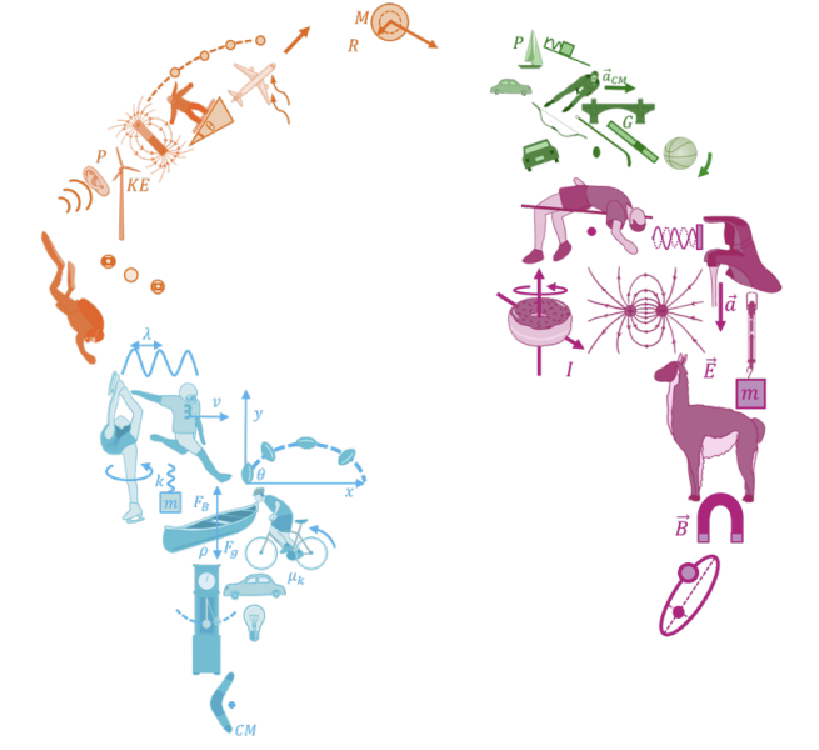
\includegraphics[width=4cm]{figures/BMDW/logo}
\end{textblock*}

\end{frame}

%%%%%%%%%%%%%TOC

\twocolframe{Outline}
{\tableofcontents[sections=1-2, subsectionstyle=show/show]\thispagestyle{empty}}
{\tableofcontents[sections=3, subsectionstyle=show/show]}

%%%%%%%%%%%%%%%%%%%%%%%%%











%%%%%%%%%%%%%%%%%%%%%%%%%%%%%%%%
\section{Angular and Rolling Motion}
\label{sec:angularandrollingmotion}
\title{Angular and Rolling Motion}
\institute{Rotational Energy, Momentum and RWS}
\author{\insertsubsection}


%%%%%%%%%%%%%%%%%%%%%%%%%
\begin{frame}
\titlepage
\thispagestyle{empty}
\end{frame}

%%%%%%%%%%%%%%%%%%%%%









\subsection{Review: Rotational Dynamics}
\label{subsec:rotationaldynamicsreview}
\twocolframe{Quick review: Rotational dynamics}
{
\begin{itemize}
\item Torque on a body \textbf{about an axis}:
\begin{align*}
\vec \tau = \vec r \times \vec F
\end{align*}
\item Rotational equivalent of Newton's Second Law:
\begin{align*}
\sum \pvec \tau^{ext}=I\vec \alpha
\end{align*}
\item Moment of inertia of an object \textbf{about an axis}:
\begin{align*}
I = \sum m_ir_i^2=\int_0^Mr^2dm
\end{align*}
\end{itemize}
}
{
\begin{itemize}
\item We describe the motion of a rotating object using kinematic quantities (position, velocity, acceleration):
\begin{align*}
\omega=\frac{d\theta}{dt}\quad\quad \alpha=\frac{d\omega}{dt}
\end{align*}
\item In order to describe about which axis these refer to, we use the right hand rule for axial vectors to define directions for corresponding vectors:
\begin{align*}
\vec \omega, \vec \alpha
\end{align*}
\end{itemize}
}


%%%%%%%%%%%%%%%%%%%%%%%%%%%%%%%%
\begin{frame} {Why introduce rotational stuff?}
\begin{itemize}
\item In the last few chapters, we have expanded our ability to build models from describing particles to ``solid objects''.
\item Newton’s Second Law only describes a point particle:
\begin{align*}
\sum \vec F = m\vec a
\end{align*}
\item By considering solid objects as being made of many point particles, we can now describe the motion of on an object as a whole:
\begin{itemize}
\item How its centre of mass moves:
\begin{align*}
\sum \pvec F^{ext} = M\vec a_{CM}
\end{align*}
\item How the object rotates about the centre of mass:
\begin{align*}
\sum \pvec \tau^{ext}=I\vec \alpha
\end{align*}
\end{itemize}
\end{itemize}
\end{frame}

%%%%%%%%%%%%%%%%%%%%%%%%%%%%%%%%
\begin{frame}{Motion, in general}
\capfig{0.5}{figures/AngularMomentumRolling/cmparabola}{The motion of the dumbbell appears complicated, but is just a combination of motion of the CM and rotation about the CM.}
Think of the motion of the dumbbell as the combination of:
\begin{enumerate}
\item Motion of the CM according to external forces (gravity $\rightarrow$ parabolic motion).
\item Uniform circular motion about the CM (no external torque).
\end{enumerate}
\end{frame}


%%%%%%%%%%%%%%%%%%%%%%%%%%%%%%%%

%%%%%%%%%%%%%%%%%%%%%%%%%%%%%%%%
\subsection{Energy of Rotating Objects}
\label{subsec:energyofarotatingobject}
\begin{frame}{Energy of an object that can rotate}
\begin{itemize}
\item It takes energy to accelerate the centre of mass. We call this ``translational kinetic energy''.
\begin{align*}
K_{trans}=\frac{1}{2}Mv_{CM}^2
\end{align*}
\item It takes energy to make the object rotate. We call this ``\textbf{rotational kinetic energ}y''. 
\begin{align*}
K_{rot}=\frac{1}{2}I\omega^2
\end{align*}
\item If an object's CM is moving, and the object is rotating, its total kinetic energy is the sum of these 2 (and \textbf{we take the axis of rotation through the CM}):
\begin{align*}
\Aboxed{K_{tot}=\frac{1}{2}Mv_{CM}^2+\frac{1}{2}I\omega^2}
\end{align*}
\end{itemize}
\end{frame}


%%%%%%%%%%%%%%%%%%%%%%%%%%%%%%%%
\twocolframesf{Work-Energy theorem}
{
\begin{itemize}
\item It takes work to give the object translational kinetic energy:
\begin{align*}
W^{net}=\int \pvec F^{net}\cdot d\vec l=\Delta K_{trans}
\end{align*}
The net force is exerted over a certain distance/displacement.

\item It takes work to give the object rotational kinetic energy:
\begin{align*}
W^{net}=\int \pvec \tau^{net}\cdot d\vec \theta=\Delta K_{rot}
\end{align*}
The net torque is exerted over a certain angular displacement.
\end{itemize}
}
{
\begin{center}
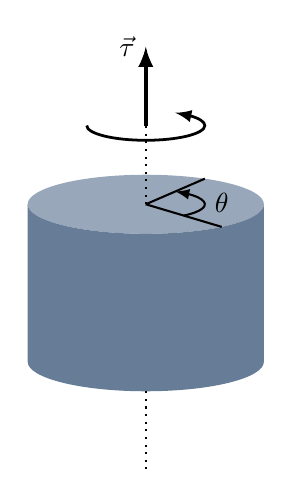
\begin{tikzpicture}[scale=1]
\tikzmath{
\R=1.5;
\h=2;
}
\scalebox{1}{

\fill[color=myblue!40] (0,0) circle ({\R} and {\R/4});
\fill[color=myblue!60] (\R,0) arc(360:180:{\R} and {\R/4}) -- (-\R,-\h) arc(180:360:{\R} and {\R/4}) --cycle;

\draw[line width=0.75] (0,0) -- (-50:{\R} and {\R/4});
\draw[line width=0.75] (0,0) -- (60:{\R} and {\R/4});
\draw[-latex, line width=0.75] (-50:{0.5*\R} and {\R/8}) arc (-50:60:{0.5*\R} and {\R/8}) node[midway,right]{$\theta$};

\draw[dotted,line width=0.75] (0,0) -- +(0,\h);
\draw[dotted,line width=0.75] (0,-\h-\R/4) -- +(0,-0.5*\h);
\draw[-latex,line width=1.5] (0,0.5*\h) --+(0,1) node[left]{$\vec \tau$};

\draw[-latex,line width=1] (-\R/2,0.5*\h) arc (180:420:{0.5*\R} and {\R/8});

}
\end{tikzpicture}
\captionof*{figure}{\textit{Work done by torque over an angular displacement.}}
\end{center}

}


%%%%%%%%%%%%%%%%%%%%%%%%%%%%%%%%



%%%%%%%%%%%%%%%%%%%%%%%%%%%%%%%%
\subsection{Rolling Motion}
\label{subsec:}
\begin{frame}{Rolling motion}
\begin{itemize}
\item<1-> A specific combination of translational and rotational motion.
\item<2-> The velocity of any point with respect to the ground is the sum of:
\begin{itemize}
\item The velocity of the CM.
\item The velocity of the point relative to the CM (with speed given by $v=\omega R$).
\end{itemize}
\item<3-> Can have rolling with or without slipping. If \textbf{without} slipping:
\begin{align*}
\Aboxed{v_{CM}=\omega R}
\end{align*}
\end{itemize}
%
\vspace{-0.75cm}
\begin{center}
\begin{tikzpicture}[scale=1]
\tikzmath{
\R=1.4;
\lvcm=1;
}
\scalebox{1}{

%wheel with spokes
\draw[line width=1.5] (0,0) circle(\R);
\fill (0,0) circle(2pt);
\foreach \th in {0,45,...,360}{
\draw (0,0) --+(\th:\R);
}
\node[above,left] at (0,0) {\scriptsize CM};
\draw[-latex,line width =2] (0,0) -- +(\lvcm,0) node[above]{\scriptsize $\vec v_{CM}$};
\draw[-latex,line width =2] (90:\R) -- +(\lvcm,0) node[above]{\scriptsize $\vec v_{CM}$};
\draw[-latex,line width =2] (270:\R) -- +(\lvcm,0) node[below]{\scriptsize $\vec v_{CM}$};

\node at (1.5*\R,0) {\Huge $+$};

\begin{scope}[shift={(3*\R,0)}]

\draw[line width=1.5] (0,0) circle(\R);
\fill (0,0) circle(2pt);
\foreach \th in {0,45,...,360}{
\draw (0,0) -- (\th:\R);
\draw [-latex, line width = 2] (\th:\R) -- +({\th-90}:\lvcm);
}
\node[above right] at (90:\R) {\scriptsize $\omega R$};

\end{scope}


\only<2,3>{
\node at (4.5*\R,0) {\Huge $=$};

\begin{scope}[shift={(6*\R,0)}]

\draw[line width=1.5] (0,0) circle(\R);
\fill (0,0) circle(2pt);
\foreach \th in {0,45,...,360}{
\draw (0,0) -- (\th:\R);
\ifthenelse{\th=270}{
\fill[color=red] (\th:\R) circle(2pt)}{
\draw [-latex, line width = 2,color=red] (\th:\R) -- ($ (\th:\R)+({\th-90}:\lvcm) +(\lvcm,0)$)};
}

\end{scope}
}
\only<4>{
\node at (4.5*\R,0) {\Huge $=$};
\node at (6*\R,0) {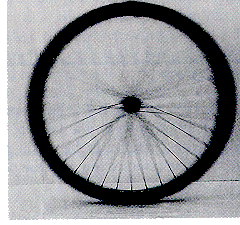
\includegraphics[scale=0.6]{figures/AngularMomentumRolling/wheel}};

}

}


\end{tikzpicture}
\captionof*{figure}{ \textit{Rolling motion. \only<2->{In rolling without slipping, the point of contact must be at rest relative to the ground.}}}
\end{center}
\end{frame}


%%%%%%%%%%%%%%%%%%%%%%%%%%%%%%%%







%%%%%%%%%%%%%%%%%%%%%%%%%%%%%%%%
\section{Rolling Without Slipping}
\label{sec:rws}
\title{Rolling Without Slipping}
\institute{Rotational Energy, Momentum and RWS}
\author{\insertsubsection}


%%%%%%%%%%%%%%%%%%%%%%%%%
\begin{frame}
\titlepage
\thispagestyle{empty}
\end{frame}

%%%%%%%%%%%%%%%%%%%%%








%%%%%%%%%%%%%%%%%%%%%%%%%%%%%%%%



%%%%%%%%%%%%%%%%%%%%%%%%%%%%%%%%


%%%%%%%%%%%%%%%%%%%%%%%%%%%%%%%%
\subsection{Modelling RWS}
\label{subsec:Modelling RWS}
\twocolframesf{Modeling rolling without slipping}
{
\only<1>{Group question}
\begin{enumerate}
\item Draw the forces on the cylinder.
\item Write the equations of motion:
\begin{itemize}
\item Sum of the forces in the $x$ direction:
\only<2>{
\begin{align*}
\sum F_x=Mg\sin\theta-f_s=Ma_{CM}
\end{align*}
}
\item Sum of the forces in the $y$ direction:
\only<2>{
\begin{align*}
\sum F_y=N-Mg\cos\theta=0
\end{align*}
}
\item Sum of the torques about the CM:
\only<2>{
\begin{align*}
\sum \tau_z=-f_sR=\frac{1}{2}MR^2\alpha
\end{align*}
}
\end{itemize}
\item<2> Can now solve for $a_{CM}, f_s, N$...
\end{enumerate}
}
{
\vspace{-1cm}
\begin{center}
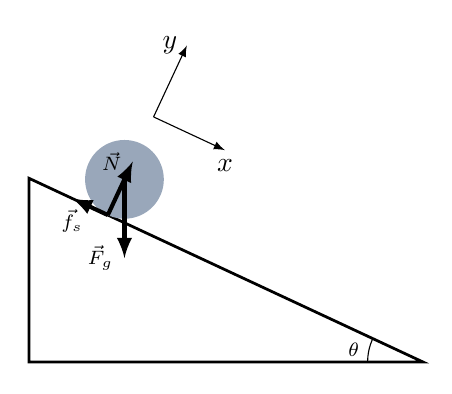
\begin{tikzpicture}[scale=1]
\tikzmath{
\L=5;
\th=25;
\h=\L*tan(\th);
\d=0.8*\L/cos(\th);
\R=0.5;
}
\scalebox{1}{

\coordinate (P) at ($(\L,0)+(180-\th:\d)$);
\coordinate (PC) at ($(P)+(90-\th:\R)$);
\coordinate (OC) at ($(P)+(90-\th:2.75*\R)$);


\draw[-latex] (OC) --+(-\th:1) node[below]{$x$};
\draw[-latex] (OC) --+(90-\th:1) node[left]{$y$};

\draw[line width=1] (0,0) -- (0,\h) -- (\L,0) -- cycle;
\fill[color=myblue!40] (PC) circle(\R);
\draw ($(\L,0)-(0.7,0)$) arc(180:180-\th:0.7) node[midway,left]{\scriptsize $\theta$};

\only<2>{
\draw[-latex, line width=1.5] (PC) -- +(0,-1) node[left]{\scriptsize $\vec F_g$};
\draw[-latex, line width=1.5] (P) -- +(180-\th:0.5) node[below]{\scriptsize $\vec f_s$};
\draw[-latex, line width=1.5] (P) -- +(90-\th:0.75) node[left]{\scriptsize $\vec N$};
}


}


\end{tikzpicture}
\captionof*{figure}{ \textit{A cylinder rolling down an incline. \only<2>{If the incline is too steep, the force of static friction cannot be large enough to prevent slipping.}}}
\end{center}
\only<2>{
For rolling without slipping:
\begin{align*}
\Aboxed{a_{CM}=\alpha R}
\end{align*}

}
}


%%%%%%%%%%%%%%%%%%%%%%%%%%%%%%%%
\subsection{Instantaneous axis of rotation}
\label{subsec:instaxisofrotation}
\begin{frame}{The instantaneous axis of rotation}
\begin{itemize}
\item In rolling \textbf{without} slipping, one can choose the instantaneous axis of rotation (through the point of contact with the ground) instead of the CM to build a model.
\item About the instantaneous axis (fixed to the ground, so inertial frame of reference), the \textbf{motion is rotation only}, not the sum of rotation and translation
\item The angular velocity is the same about the CM or about the instantaneous axis!
\end{itemize}
\begin{center}
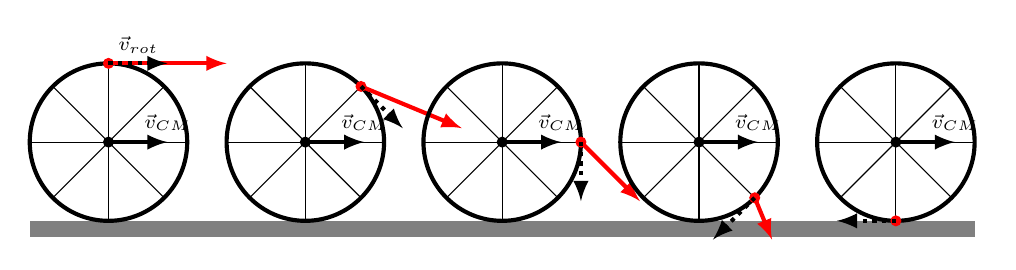
\begin{tikzpicture}[scale=1]
\tikzmath{
\R=1;
\lvcm=0.75;
}
\scalebox{1}{

\fill[color=black!50] (-\R,-\R-0.2) rectangle (11*\R,-\R);

%wheel with spokes

\foreach \x/\thth in{0/90,2.5*\R/45,5*\R/0,7.5*\R/-45,10*\R/-90}{

\draw[line width=1.5] (\x,0) circle(\R);
\fill (\x,0) circle(2pt);
\foreach \th in {0,45,...,360}{
\draw (\x,0) --+(\th:\R);
}

\draw[-latex,line width =1.5] (\x,0) -- +(\lvcm,0) node[above]{\scriptsize $\vec v_{CM}$};
\fill[color=red] ($(\x,0)+(\thth:\R)$) circle(2pt);


\ifthenelse{\thth=-90}{}{%don't draw the bottom one because it screws up the arrow of length 0
\draw [-latex, line width = 1.5,color=red] ($(\x,0)+(\thth:\R)$) -- ($ (\x,0)+(\thth:\R)+({\thth-90}:\lvcm)+(\lvcm,0)$)};

\draw [-latex, line width = 1.5, dotted]($(\x,0)+(\thth:\R)$) -- ($ (\x,0)+(\thth:\R)+({\thth-90}:\lvcm)$);
\ifthenelse{\thth=90}{\node[above right] at (0,\R) {\scriptsize $\vec v_{rot}$}}{};
}


}

\end{tikzpicture}
\captionof*{figure}{\textit{In rolling without slipping any point on the wheel can be modeled as rotating about the point of contact with the ground.}}
\end{center}
\end{frame}


%%%%%%%%%%%%%%%%%%%%%%%%%%%%%%%%
\twocolframesf{The instantaneous axis of rotation}
{
\begin{itemize}
\item About the instantaneous axis of rotation, each point is at a different distance from the axis.
\item The velocity vector for any point is perpendicular to $\vec r$ and to $\vec \omega$. It is given by:
\begin{align*}
\vec v =\vec \omega \times \vec r
\end{align*}
\item For example, the speed of the CM is given by:
\begin{align*}
v_{CM}=||\vec \omega \times \vec r_{CM}||=\omega R
\end{align*}
Which is the speed of the CM relative to the ground. \textbf{The angular velocity must be the same about the CM and about the instantaneous axis}.
\end{itemize}
}
{
\only<1>{
\begin{center}
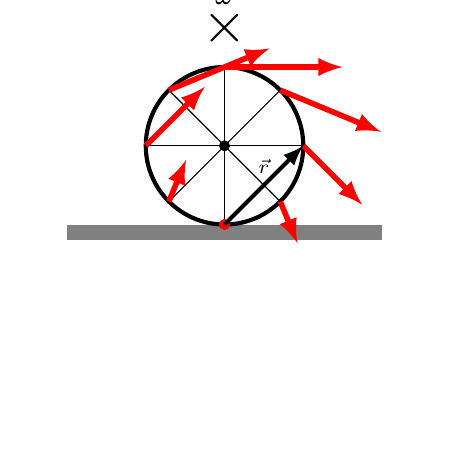
\begin{tikzpicture}[scale=1]
\tikzmath{
\R=1;
\lvcm=0.75;
}
\useasboundingbox (-2.5*\R,-2.5*\R) rectangle (2.5*\R,2.5*\R);
\scalebox{1}{
\node at (0,2.5*\R) {\huge $\times$};
\node[above=5pt] at (0,2.5*\R) {$\vec \omega$};

\fill[color=black!50] (-2*\R,-0.2) rectangle (2*\R,0);

\draw[line width=1.5] (0,\R) circle(\R);
\fill (0,\R) circle(2pt);

\foreach \th in {45,90,...,360}{
  \draw (0,\R) -- ($(0,\R)+(\th:\R)$);
  \ifthenelse{\th=270}{
    \fill[color=red] ($(0,\R)+(\th:\R)$) circle(2pt)}{
    \draw [-latex, line width = 2,color=red] ($(0,\R)+(\th:\R)$) -- ($ (0,\R)+(\th:\R)+({\th-90}:\lvcm) +(\lvcm,0)$)
  };
 \ifthenelse{\th=360}{
   \draw [-latex, line width = 1.5](0,0) -- ($(0,\R)+(\th:\R)$) node[midway,above]{\scriptsize $\vec r$};
  }{}; 
}
}

\end{tikzpicture}
\captionof*{figure}{\textit{About the instantaneous axis of rotation, all points appear to rotate around the axis with the same angular velocity.}}
\end{center}}

\only<2>{
\begin{center}


\begin{animateinline}[autoplay,loop]{5} % 5 fps, same as 0.2 s transduration

\multiframe{24}{i=0+1}{

\begin{tikzpicture}[scale=1]

\tikzmath{
\R=1;
\lvcm=0.75;
\rotangle=\i*15;
\rcirc=sqrt(2)*\R;
}
\useasboundingbox (-2.5*\R,-2.5*\R) rectangle (2.5*\R,2.5*\R);
\scalebox{1}{

\draw[dashed] (0,0) circle(\rcirc);

\fill[color=black!50] (-2*\R,-0.2) rectangle (2*\R,0);
\fill[color=red] (0,0) circle(2pt);

\begin{scope}[rotate=-\rotangle]
\draw[line width=1.5] (0,\R) circle(\R);
\fill (0,\R) circle(2pt);

\foreach \th in {45,90,...,360}{
  \draw (0,\R) -- ($(0,\R)+(\th:\R)$); 
  \ifthenelse{\th=270}{
    \fill[color=red] ($(0,\R)+(\th:\R)$) circle(2pt)}{
    \draw [-latex, line width = 2,color=red] ($(0,\R)+(\th:\R)$) -- ($ (0,\R)+(\th:\R)+({\th-90}:\lvcm) +(\lvcm,0)$)
  };
}
\end{scope}
}
\end{tikzpicture}
%%%% end animate
}
\end{animateinline}


\captionof*{figure}{\textit{About the instantaneous axis of rotation, all points appear to rotate around the axis with the same angular velocity.}}

\end{center}
}

}


%%%%%%%%%%%%%%%%%%%%%%%%%%%%%%%%
\subsection{Modeling RWS with inst. axis}
\label{subsec:}
\twocolframesf{Modeling rolling without slipping about the instantaneous axis}
{
\begin{enumerate}
\item Draw the forces on the cylinder.
\item Write the equations of motion:
\begin{itemize}
\item Sum of the forces in the $x,y$ directions (unchanged):
\begin{align*}
\sum F_x&=Mg\sin\theta-f_s=Ma_{CM}\\
\sum F_y&=N-Mg\cos\theta=0
\end{align*}
\item Sum of the torques about the point of contact (\textbf{use parallel axis theorem} for $I$!):
\begin{align*}
\sum \tau_z=-Mg\sin\theta R=\left(\frac{1}{2}MR^2+MR^2\right)\alpha
\end{align*}
\end{itemize}
\item Can immediately determine $\alpha$ ($a_{CM}$) in this case!
\end{enumerate}
}
{
\vspace{-0.5cm}
\begin{center}
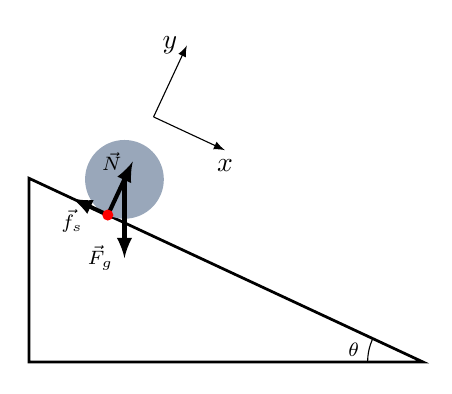
\begin{tikzpicture}[scale=1]
\tikzmath{
\L=5;
\th=25;
\h=\L*tan(\th);
\d=0.8*\L/cos(\th);
\R=0.5;
}
\scalebox{1}{

\coordinate (P) at ($(\L,0)+(180-\th:\d)$);
\coordinate (PC) at ($(P)+(90-\th:\R)$);
\coordinate (OC) at ($(P)+(90-\th:2.75*\R)$);

\draw[-latex] (OC) --+(-\th:1) node[below]{$x$};
\draw[-latex] (OC) --+(90-\th:1) node[left]{$y$};

\draw[line width=1] (0,0) -- (0,\h) -- (\L,0) -- cycle;
\fill[color=myblue!40] (PC) circle(\R);
\draw ($(\L,0)-(0.7,0)$) arc(180:180-\th:0.7) node[midway,left]{\scriptsize $\theta$};

\draw[-latex, line width=1.5] (PC) -- +(0,-1) node[left]{\scriptsize $\vec F_g$};
\draw[-latex, line width=1.5] (P) -- +(180-\th:0.5) node[below]{\scriptsize $\vec f_s$};
\draw[-latex, line width=1.5] (P) -- +(90-\th:0.75) node[left]{\scriptsize $\vec N$};
\fill[color=red] (P) circle(2pt);
}


\end{tikzpicture}
\captionof*{figure}{ \textit{A cylinder rolling down an incline, modeled using instantaneous axis of rotation.}}
\end{center}

For rolling without slipping:
\begin{align*}
\Aboxed{a_{CM}=\alpha R}
\end{align*}

}


%%%%%%%%%%%%%%%%%%%%%%%%%%%%%%%%



%%%%%%%%%%%%%%%%%%%%%%%%%%%%%%%%
\subsection{Example: giant yo-yo}
\label{subsec:giantyoyoexample}
\twocolframesf{Example: Giant Yo-Yo}
{

\only<2>{
\begin{itemize}
\item The direction of motion of the yo-yo depends on the angle with which we pull the rope
\item The direction of the force of friction is tricky to determine!
\item When the angle is low:
\begin{itemize}
\item The yo-yo goes towards the right (towards F).
\item $\vec f_s$ has to be towards the left so that the net torque about the CM is into the page. (The torque from F about the CM would make the wheel go to the left).
\end{itemize}

\end{itemize}
}
\only<3>{
\begin{itemize}
\item Sum of forces:
\begin{align*}
\sum F_x &= F\cos\theta -f_s=Ma_{CM}\\
\sum F_y &= F\sin\theta+N-Mg=0
\end{align*}
\item Sum of torques \textbf{about CM} (only $\vec F$ and $\vec f_s$):
\begin{align*}
\sum \tau_z= FR_1-f_sR_2=I\alpha
\end{align*}
\end{itemize}
\vspace{-0.5cm}
\begin{block}{Thinking about it}
\begin{itemize}
\item When the angle is small, the torque about CM from $\vec f_s$ is larger than that from $\vec F$ (yo-yo goes to the right)
\item Above some angle, the torque from $\vec f_s$ is less than that from $\vec F$ and the yo-yo goes the other way.
\item There is an angle where the net torque is zero $\rightarrow$ the yo-yo just slides
\end{itemize}
\end{block}

}

}
{
\vspace{-1cm}
\begin{center}
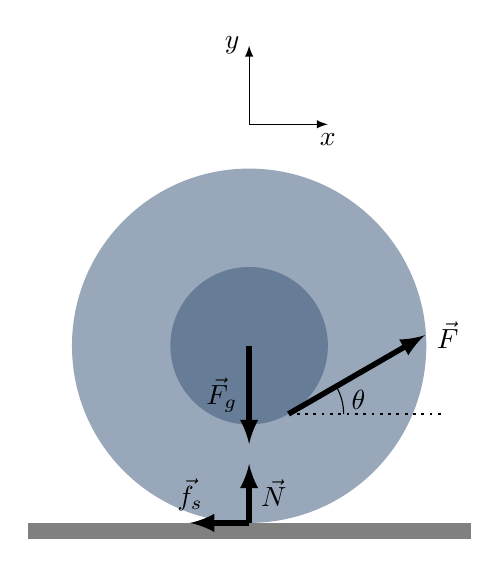
\begin{tikzpicture}[scale=1]
\tikzmath{
\Rb=2.25;
\Rs=1;
\th=30;
\fl=2;
}
\scalebox{1}{

\coordinate (P) at ($(0,\Rb)+(270+\th:\Rs)$);
\coordinate (OC) at (0,2.25*\Rb);

\draw[-latex] (OC) -- +(1,0) node[below]{$x$};
\draw[-latex] (OC) -- +(0,1) node[left]{$y$};

\fill[black!50] (-1.25*\Rb,-0.2) rectangle (1.25*\Rb,0);

\fill[myblue!40] (0,\Rb) circle(\Rb);
\fill[myblue!60] (0,\Rb) circle(\Rs);

\draw[-latex,line width=2] (P) -- +(\th:\fl) node[right]{$\vec F$};
\draw[dotted,line width=1] (P) -- +(2,0);
\draw ($(P) +(0.7,0)$) arc (0:\th:0.7) node[midway,right]{$\theta$};

\only<2->{
\draw[-latex,line width=2] (0,0) -- +(0,0.75) node[midway,right]{$\vec N$};
\draw[-latex,line width=2] (0,\Rb) -- +(0,-1.25) node[midway,left]{$\vec F_g$};
\draw[-latex,line width=2] (0,0) -- +(-0.75,0) node[above]{$\vec f_s$};
}

}


\end{tikzpicture}
\captionof*{figure}{ \textit{Modeling a giant yo-yo.}}
\end{center}
}

%%%%%%%%%%%%%%%%%%%%%%%%%%%%%%%%



%%%%%%%%%%%%%%%%%%%%%%%%%%%%%%%%





%%%%%%%%%%%%%%%%%%%%%%%%%%%%%%%%
\section{Angular Momentum}
\label{sec:angularmomentum}
\title{Angular Momentum}
\institute{Rotational Energy, Momentum and RWS}
\author{\insertsubsection}


%%%%%%%%%%%%%%%%%%%%%%%%%
\begin{frame}
\titlepage
\thispagestyle{empty}
\end{frame}

%%%%%%%%%%%%%%%%%%%%%





%%%%%%%%%%%%%%%%%%%%%%%%%%%%%%%%
\subsection{Formula}
\label{subsec:formulaangmomentum}
\twocolframest{Rotational dynamics – angular momemtum}
{
\begin{itemize}
\item Given an axis of rotation:
\begin{align*}
\vec r \times (\pvec F^{net} &= m\vec a)\\
\therefore \pvec \tau^{net} &=mr^2\alpha
\end{align*}
\item Rotational version of momentum (angular momentum):
\begin{align*}
\vec L&=\vec r \times \vec p\\
\frac{d\vec L}{dt}&=\frac{d}{dt} (\vec r \times \vec p) = \cancelto{0\;\;(\vec v \parallel \vec p)}{\frac{d\vec r}{dt}\times \vec p} + \vec r \times\frac{d\vec p }{dt}=\pvec \tau^{net} \\
\therefore \Aboxed{\frac{d\vec L}{dt}&=\pvec \tau^{net}} \quad\quad \text{compare to}\quad\quad \frac{d\vec p}{dt}=\pvec F^{net}
\end{align*}
\end{itemize}

}
{
\begin{center}
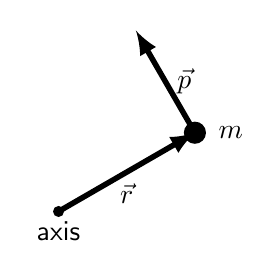
\begin{tikzpicture}[scale=1]
\tikzmath{}
\scalebox{1}{

\fill (0,0) circle (2pt) node[below]{axis};

\draw[-latex,line width = 2] (0,0) -- (30:2) node[midway, below]{$\vec r$};
\fill (30:2) circle (4pt) node[right=5pt]{$m$};
\draw[-latex,line width = 2] (30:2) -- +(120:1.5) node[midway, right]{$\vec p$};

}

\end{tikzpicture}
\captionof*{figure}{\textit{Angular momentum is defined for a particular axis of rotation based on the particle's momentum.}}
\end{center}
}


%%%%%%%%%%%%%%%%%%%%%%%%%%%%%%%%
\subsection{Expressing angular momentum}
\label{subsec:}
\twocolframest{Angular momentum of particle}
{
\begin{itemize}
\item If there is \textbf{no net torque} about an axis on the mass, then its \textbf{angular momentum relative to that axis is conserved}.
\item There could be a net force on the particle (momentum is not conserved), but if the net force is in such a way that it produces no net torque (\textbf{about a given point}), then angular momentum (\textbf{about that given point}) is conserved.
\item Angular momentum measures how much ``rotation'' a particle has about a particular axis. 
\item[$\rightarrow$] If the particle has no angular velocity about that axis, it has no angular momentum about that axis.
\item[$\rightarrow$] If the particle is further from axis or more massive, it has more angular momentum.
\end{itemize}
}
{
\begin{center}
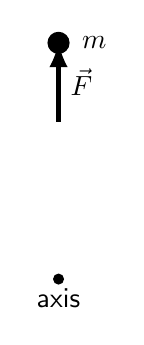
\begin{tikzpicture}[scale=1]
\tikzmath{}
\scalebox{1}{

\fill (0,0) circle (2pt) node[below]{axis};
\fill (90:3) circle (4pt) node[right=5pt]{$m$};


\draw[latex-,line width = 2] (90:3) -- +(0,-1)  node[midway, right]{$\vec F$};



}

\end{tikzpicture}
\captionof*{figure}{\textit{In this case, linear momentum is not conserved while angular momentum about the given axis is conserved.}}
\end{center}
}


%%%%%%%%%%%%%%%%%%%%%%%%%%%%%%%%
\twocolframest{Angular momentum of a system}
{
\begin{itemize}
\item We summed the momenta of the particles in a system:
\begin{align*}
\frac{d\vec p_i}{dt}&=\pvec F^{net}\\
\therefore \frac{d\vec P}{dt}&=\pvec F^{ext}
\end{align*}
\item We do the same for angular momentum:
\begin{align*}
\frac{d\vec L_i}{dt}&=\pvec \tau^{net}\\
\therefore \frac{d\vec L}{dt}&=\pvec \tau^{ext}
\end{align*}
\item If there is \textbf{no net external torque on a system}, the angular momentum of the system is conserved
\end{itemize}
}
{
\begin{center}
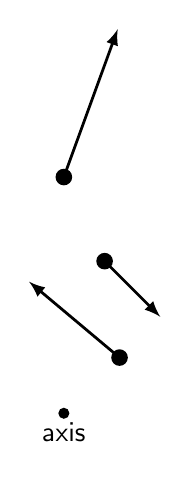
\begin{tikzpicture}[scale=1]
\tikzmath{}
\scalebox{1}{

\fill (0,0) circle (2pt) node[below]{axis};
\fill (90:3) circle (3pt);
\draw[-latex,line width = 1] (90:3) -- +(70:2);

\fill (45:1) circle (3pt);
\draw[-latex,line width = 1] (45:1) -- +(140:1.5);

\fill (75:2) circle (3pt);
\draw[-latex,line width = 1] (75:2) -- +(-45:1);
}

\end{tikzpicture}
\captionof*{figure}{\textit{The total angular momentum is the sum of the angular momenta of the particles in the system.}}
\end{center}
}


%%%%%%%%%%%%%%%%%%%%%%%%%%%%%%%%
\begin{frame}{Angular momentum for a solid object}
\begin{itemize}
\item For a single particle in a system its angular momentum about an axis of rotation is:
\begin{align*}
\vec L_i = \vec r_i\times \vec p_i = \vec r_i \times m_i\vec v_i=m_i \vec r_i \times (\vec \omega \times\vec r_i)=m_ir_i^2\vec \omega
\end{align*}
\item Adding together the angular momenta of particles in a solid object (all with the same angular velocity):
\begin{align*}
\vec L &= \left(\sum_i m_ir_i^2 \right) \vec \omega\\
\Aboxed{\vec L &=I\vec\omega}
\end{align*}
\end{itemize}

\end{frame}


%%%%%%%%%%%%%%%%%%%%%%%%%%%%%%%%
\subsection{Angular in relation to linear quantities}
\label{subsec:correspondencetable}
\begin{frame}{Correspondence between linear and angular}
\begin{tabular}{llll}
\textbf{Name} &\textbf{Linear} & \textbf{Angular} & \textbf{Correspondence}\\
\hline\hline
Displacement & $s$ & $\vec \theta$ & $d\vec\theta=\frac{1}{r^2} \vec r\times d\vec s$  \\
Velocity & $\vec v$ & $\vec \omega$ & $\vec\omega=\frac{1}{r^2} \vec r\times \vec v$, $v_T = \vec\omega\times \vec r$ \footnote{This corresponds to the component of velocity perpendicular to $\vec r$.}\\
Acceleration & $\vec a$ & $\vec \alpha$ & $\vec\alpha=\frac{1}{r^2} \vec r\times \vec a$, $a_T = \vec\alpha\times \vec r$ \footnote{This corresponds to the component of acceleration perpendicular to $\vec r$.}\\
Inertia& $m$ & $I$ & $I=\sum_i m_ir_i^2$ \\
Momentum& $\vec p=m\vec v$& $\vec L = I\vec \omega$ &$\vec L = \vec r\times \vec p$ \\
Newton's Second Law&$\pvec F^{ext}=m\vec a_{CM}$ & $\pvec \tau^{ext} = I\vec\alpha$& $\vec F \to \vec\tau$, $m\to I$, $\vec a \to \vec \alpha$\\
Newton's Second Law& $\frac{d\vec p}{dt} =\pvec F^{ext}$ & $\frac{d\vec L}{dt} =\pvec \tau^{ext}$&$\vec F \to \vec\tau$, $\vec p \to \vec L$ \\
Kinetic energy&$\frac{1}{2}mv^2$ &$\frac{1}{2}I\omega^2$ &$m\to I$, $v\to \omega$ \\
Power&$\vec F \cdot \vec v$ &$\vec \tau \cdot \vec\omega$ &$\vec F \to \vec\tau$, $\vec v\to \vec\omega$  \\
\end{tabular}
\end{frame}


%%%%%%%%%%%%%%%%%%%%%%%%%%%%%%%%


%%%%%%%%%%%%%%%%%%%%%%%%%%%%%%%%
\subsection{Planets and the solar system}
\label{subsec:planets and the solar system}
\twocolframesf{Planets and the solar system}
{
\begin{itemize}
\item The solar system started off as a very big roughly spherical ball of gas with atoms moving in all directions.
\item Since the motion of the atoms was random, there was a net total angular momentum in some direction.
\item Atoms and matter coalesced because of gravity towards the centre of mass:
\begin{itemize}
\item Their rotational speed had to increase (moment of inertia got smaller).
\item They all ended up in the same plane (perpendicular to angular momentum of the system), mostly due to collisions.
\end{itemize}
\end{itemize}
}{
\capfig{1}{figures/AngularMomentumRolling/solarsystem}{Through conservation of angular momentum, all planet orbit in a similar plane. \scriptsize \url{https://jcconwell.wordpress.com/tag/angular-momentum/}}
}

%%%%%%%%%%%%%%%%%%%%%%%%%%%%%%


%%%%%%%%%%%%%%%%%%%%%%%%%%%%%%%%

%%%%%%%%%%%%%%%%%%%%%%%%%%%%%%%%
\subsection{Example: bicycle wheel}
\label{subsec:bicyclewheelexample}
\twocolframe{Example: Bicycle wheel}
{Tilt the axis of the wheel!}
{

\begin{center}
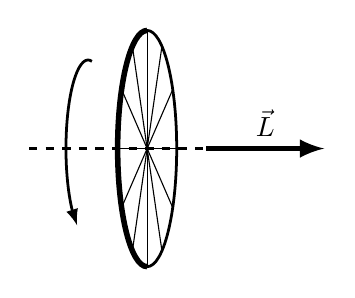
\begin{tikzpicture}[scale=1]
\tikzmath{
\R=1.5;
}
\scalebox{1}{

\draw[-latex, line width=1] ($(-0.5*\R,0)+(80:{0.75*\R/4} and {0.75*\R})$) arc (80:240:{0.75*\R/4} and {0.75*\R});
\draw[line width=1,dashed] (-\R,0) -- (\R,0);
\draw[line width=1] (0,0) circle(\R/4 and \R);
\draw[line width=2] (0,\R) arc (90:270:\R/4 and \R);
\foreach \th in {0,30,...,330}{
\draw (0,0) -- (\th:\R/4 and \R);
}
\draw[-latex,line width=2] (0.5*\R,0) -- +(\R,0) node[midway,above]{$\vec L$};

}

\end{tikzpicture}

\end{center}
}



%%%%%%%%%%%%%%%%%%%%%%%%%%%%%%%%
\twocolframefs{Tilting the bicycle wheel requires exerting a torque}
{
\begin{itemize}
\item If you try to change the axis of rotation, you have to exert a torque to change the angular momentum.
\begin{align*}
\vec \tau = \frac{d\vec L}{dt}\sim\frac{\Delta\vec L}{\Delta  t}
\end{align*}
\item If you let the wheel hang, gravity tries to rotate the axis of rotation $\rightarrow$ precession.
\end{itemize}
}
{
\begin{center}
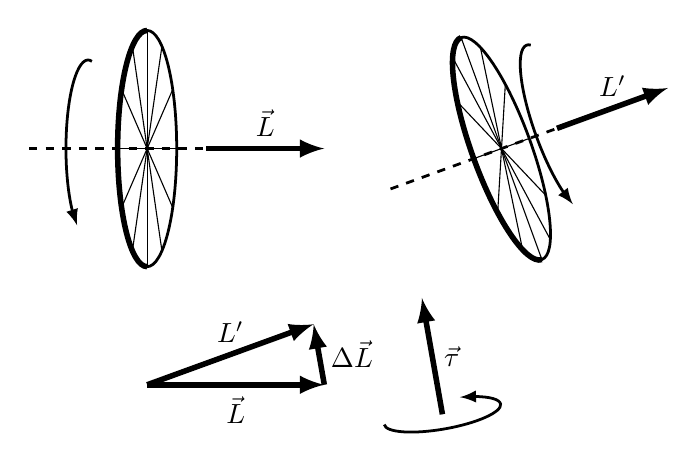
\begin{tikzpicture}[scale=1]
\tikzmath{
\R=1.5;
\throt=20;
}
\scalebox{1}{

\draw[-latex, line width=1] ($(-0.5*\R,0)+(80:{0.75*\R/4} and {0.75*\R})$) arc (80:240:{0.75*\R/4} and {0.75*\R});
\draw[line width=1,dashed] (-\R,0) -- (\R,0);
\draw[line width=1] (0,0) circle(\R/4 and \R);
\draw[line width=2] (0,\R) arc (90:270:\R/4 and \R);
\foreach \th in {0,30,...,330}{
\draw (0,0) -- (\th:\R/4 and \R);
}
\draw[-latex,line width=2] (0.5*\R,0) -- +(\R,0) node[midway,above]{$\vec L$};


\begin{scope}[shift={(3*\R,0)},rotate=\throt]
\draw[line width=1,dashed] (-\R,0) -- (\R,0);
\draw[line width=1] (0,0) circle(\R/4 and \R);
\draw[line width=2] (0,\R) arc (90:270:\R/4 and \R);
\foreach \th in {0,30,...,330}{
\draw (0,0) -- (\th:\R/4 and \R);
}
\draw[-latex,line width=2] (0.5*\R,0) -- +(\R,0) node[midway,above]{$\pvec L'$};
\draw[-latex, line width=1] ($(0.5*\R,0)+(80:{0.75*\R/4} and {0.75*\R})$) arc (80:240:{0.75*\R/4} and {0.75*\R});
\end{scope}

\begin{scope}[shift={(0,-2*\R)}]

\draw[-latex,line width=2] (0,0) -- +(1.5*\R,0) node[midway,below]{$\vec L$};
\draw[-latex,line width=2] (0,0) -- +(\throt:1.5*\R) node[midway,above]{$\pvec L'$};
\draw[-latex,line width=2] (1.5*\R,0) -- (\throt:1.5*\R) node[midway,right]{$\Delta \vec L $};

\draw[-latex,line width=2] (2.5*\R,-0.25*\R) -- +({90+\throt/2}:\R) node[midway,right]{$\vec \tau$};
\begin{scope}[shift={(2.5*\R,-0.25*\R)},rotate={\throt/2}]
\draw[-latex, line width=1] ($(0,0)+(180:{0.5*\R} and {0.5*\R/4})$) arc (180:430: {0.5*\R} and {0.5*\R/4});
\end{scope}

\end{scope}

}

\end{tikzpicture}
\captionof*{figure}{\textit{Tilting the horizontal axis of a spinning wheel requires a torque in the vertical direction!}}
\end{center}
}

%%%%%%%%%%%%%%%%%%%%%%%%%%%%%%%%



%%%%%%%%%%%%%%%%%%%%%%%%%%%%%%%%



%%%%%%%%%%%%%%%%%%%%%%%%%%%%%%%%



%%%%%%%%%%%%%%%%%%%%%%%%%%%%%%%%



%%%%%%%%%%%%%%%%%%%%%%%%%%%%%%%%



%%%%%%%%%%%%%%%%%%%%%%%%%%%%%%%%



%%%%%%%%%%%%%%%%%%%%%%%%%%%%%%%%



%%%%%%%%%%%%%%%%%%%%%%%%%%%%%%%%



%%%%%%%%%%%%%%%%%%%%%%%%%%%%%%%%



%%%%%%%%%%%%%%%%%%%%%%%%%%%%%%%%



%%%%%%%%%%%%%%%%%%%%%%%%%%%%%%%%



%%%%%%%%%%%%%%%%%%%%%%%%%%%%%%%%



%%%%%%%%%%%%%%%%%%%%%%%%%%%%%%%%






\end{document}
